\chapter{Implementation track}
\label{chap:track-implem}

\vspace{2em}
\textbf{Original title:} ZKProof Standards Implementation Track Proceedings

\textbf{Date:} 1 August 2018 + subsequent revisions

{\itshape\centering
{\color{ongoingred} This document is an ongoing work in progress.}\\
{\color{ongoingred} Feedback and contributions are encouraged.}\\
}

\vspace{1em}
\textbf{Track chairs:} 
Sean Bowe, Kobi Gurkan, Eran Tromer

\textbf{Track participants:} 
Benedikt Bünz, Konstantinos Chalkias, Daniel Genkin, Jack Grigg, Daira Hopwood, Jason Law, Andrew Poelstra, abhi shelat, Muthu Venkitasubramaniam, Madars Virza, Riad S. Wahby, Pieter Wuille



%%%%%%%%%%%%%%%%%%%%%%%%%%%%%%%%%%%%%%%%%%%%%%%%%%%%%%%%%%%%
%%%%%%%%%%%%%%%%%%%%%%%%%%%%%%%%%%%%%%%%%%%%%%%%%%%%%%%%%%%%https://www.overleaf.com/read/vhkqknmzxqvk
\section{Overview}
\label{implem:overview}
 
By having a standard or framework around the implementation of ZKPs, we aim to help platforms adapt more easily to new constructions and new schemes, that may be more suitable because of efficiency, security or application-specific changes. 
Application developers and the designers of new proof systems all want to understand the performance and security tradeoffs of different ZKP constructions when invoked in various applications. This track focuses on building a standard interface that application developers can use to interact with ZKP proof systems, in an effort to improve facilitate interoperability, flexibility and performance comparison.
In this first effort to achieve such an interface, our focus is on non-interactive proof systems (NIZKs) for general statements (NP) that use an R1CS/QAP-style constraint system representation. This includes many, though not all, of the practical general-purpose ZKP schemes currently deployed. While this focus allows us to define concrete formats for interoperability, we recognize that additional constraint system representation styles (e.g., arithmetic and Boolean circuits) are in use, and are within scope of the ongoing effort.
We also aim to establish best practices for the deployment of these proof systems in production software.


%%%%%%%%%%%%%%%%%%%%%%%%%%%%%%
\subsection{What this document is NOT about:}
\begin{itemize}
 \item A unique explanation of how to build ZKP applications
 \item An exhaustive list of the security requirements needed to build a ZKP system
 \item A comparison of front-end tools
 \item A show of preference for some use-cases or others
\end{itemize}

%%%%%%%%%%%%%%%%%%%%%%%%%%%%%%%%%%%%%%%%%%%%%%%%%%%%%%%%%%%%
%%%%%%%%%%%%%%%%%%%%%%%%%%%%%%%%%%%%%%%%%%%%%%%%%%%%%%%%%%%%
\section{Backends: Cryptographic System Implementations}
\label{implem:backends}

The backend of a ZK proof implementation is the portion of the software that contains an implementation of the low-level cryptographic protocol. It proves statements where the instance and witness are expressed as variable assignments, and relations are expressed via low-level languages (such as arithmetic circuits, Boolean circuits, R1CS/QAP constraint systems or arithmetic constraint satisfaction problems).

The backend typically consists of a concrete implementation of the ZK proof system(s) given as pseudocode in a corresponding publication (see the \hyperref[chap:track-security]{Security Track} document for extensive discussion of these), along with supporting code for the requisite arithmetic operations, serialization formats, tests, benchmarking etc.

There are numerous such backends, including implementations of many of the schemes discussed in the \hyperref[chap:track-security]{Security Track}. 
Most have originated as academic research prototypes, and are available as open-source projects. 
Since the offerings and features of backends evolve rapidly, we refer the reader to the curated taxonomy at https://zkp.science for the latest information.

Considerations for the choice of backends include:

\begin{itemize}
\item ZK proof system(s) implemented by the backend, and their associated security, assumptions and asymptotic performance (as discussed in the Security Track document)
\item Concrete performance (see Benchmarks section)
\item Programming language and API style (this consideration may be satisfied by adherence to prospective ZK proof standards; see the the API and File Formats section)
\item Platform support
\item Availability as open source
\item Active community of maintainers and users
\item Correctness and robustness of the implementation (as determined, e.g., by auditing and formal verification)
\item Applications (as evidence of usability and scrutiny).
\end{itemize}


%%%%%%%%%%%%%%%%%%%%%%%%%%%%%%%%%%%%%%%%%%%%%%%%%%%%%%%%%%%%
%%%%%%%%%%%%%%%%%%%%%%%%%%%%%%%%%%%%%%%%%%%%%%%%%%%%%%%%%%%%
\section{Frontends: Constraint-System Construction}
\label{implem:frontends}

The frontend of a ZK proof system implementation provides means to express statements in a convenient language and to prove such statements in zero knowledge by compiling them into a low-level representation and invoking a suitable ZK backend.

A frontend consists of:
\begin{itemize}
\item The specification of a high-level language for expressing statements.
\item A compiler that converts relations expressed in the high-level language into the low-level relations suitable for some backend(s). For example, this may produce an R1CS constraint system.
\item Instance reduction: conversion of the instance in a high-level statement to a low-level instance (e.g., assignment to R1CS instance variables).
\item Witness reduction: conversion of the witness to a high-level statement to a low-level witness (e.g., assignment to witness variables).
\item Typically, a library of "gadgets" consisting of useful and hand-optimized building blocks for statements.
\end{itemize}		

Languages for expressing statements, which have been implemented in frontends to date include: code library for general-purpose languages, domain-specific language, suitably-adapted general-purpose high-level language, and assembly language for a virtual CPU.

Frontends’ compilers, as well as gadget libraries, often implement various optimizations aiming to reduce the cost of the constraint systems (e.g., the number of constraints and variables). This includes techniques such as making use of “free linear combinations” in R1CS, using nondeterministic advice given in witness variables (e.g., for integer arithmetic or random-access memory), removing redundancies, using cryptographic schemes tailored for the given algebraic settings (e.g., Pedersen hashing on the Jubjub curve or MiMC for hash functions, RSA verification for digital signatures), and many other techniques. See the \href{https://docs.google.com/document/d/1aZ1GUAJOBFuqD4GOo9HqAH8w4xJo7HM4Bjte5-wkdnU/edit?usp=sharing}{Zcon0 Circuit Optimisation handout} for further discussion.

There are many implemented frontends, including some that provide alternative ways to invoke the same underlying backends. Most have originated as academic research prototypes, and are available as open-source projects. Since the offerings and features of frontends evolve rapidly, we refer the reader to the curated taxonomy at \myurl{https://zkp.science} for the latest information.


%%%%%%%%%%%%%%%%%%%%%%%%%%%%%%%%%%%%%%%%%%%%%%%%%%%%%%%%%%%%
%%%%%%%%%%%%%%%%%%%%%%%%%%%%%%%%%%%%%%%%%%%%%%%%%%%%%%%%%%%%
\section{APIs and File Formats}
\label{implem:apis-and-file-formats}

Our primary goal is to improve interoperability between proving systems and frontend consumers of proving system implementations. We focused on two approaches for building standard interfaces for implementations:

\begin{enumerate}
\item We aim to develop a common API for proving systems to expose their capabilities to frontends in a way that is maximally agnostic to the underlying implementation details.
\item We aim to develop a file format for encoding a popular form of constraint systems (namely R1CS), and its assignments, so that proving system implementations and frontends can interact across language and API barriers.
\end{enumerate}

We did not aim to develop standards for interoperability between backends implementing the same (abstract) scheme, such as serialization formats for proofs (see the Extended Constraint-System Interoperability section for further discussion).


%%%%%%%%%%%%%%%%%%%%%%%%%%%%%%
\subsection{Generic API}

In order to help compare the performance and usability tradeoffs of proving system implementations, frontend application developers may wish to interact with the underlying proof systems via a generic interface, so that proving systems can be swapped out and the tradeoffs observed in practice. 
This also helps in an academic pursuit of analysis and comparison.

The abstract parties and objects in a NIZK are %as follows:
depicted in \reffig{fig:abstract-parties-and-objects-in-NIZK}.



\begin{figure}[H]\def\tmpfigcap{Abstract parties and objects in a NIZK}
\begin{center}
\refstepcounter{figure}\label{fig:abstract-parties-and-objects-in-NIZK}%
\hypertarget{ht:figure:\thefigure}{}
\addcontentsline{lof}{figure}{Figure~\thefigure{}: \tmpfigcap}
{
\bookmarksetup{level=3,color=\colorbkmfig}
\bookmark[dest=ht:figure:\thefigure]{Figure~\thefigure}%
\internallinenumbers
{
\nolinenumbers
\def\figlang{\hyperlink{def:language}{\scalebox{.75}{Language}}}
\def\figgen{Gen}
\def\figpp{pp}
\def\figwitness{\hyperlink{def:witness}{Witness}}
\def\figinstance{\hyperlink{def:instance}{Instance}}
\def\figprover{Prover}
\def\figproof{Proof}
\def\svgwidth{.99\textwidth}
\input{figs/implem--api-diagram.pdf_tex}
}
}
%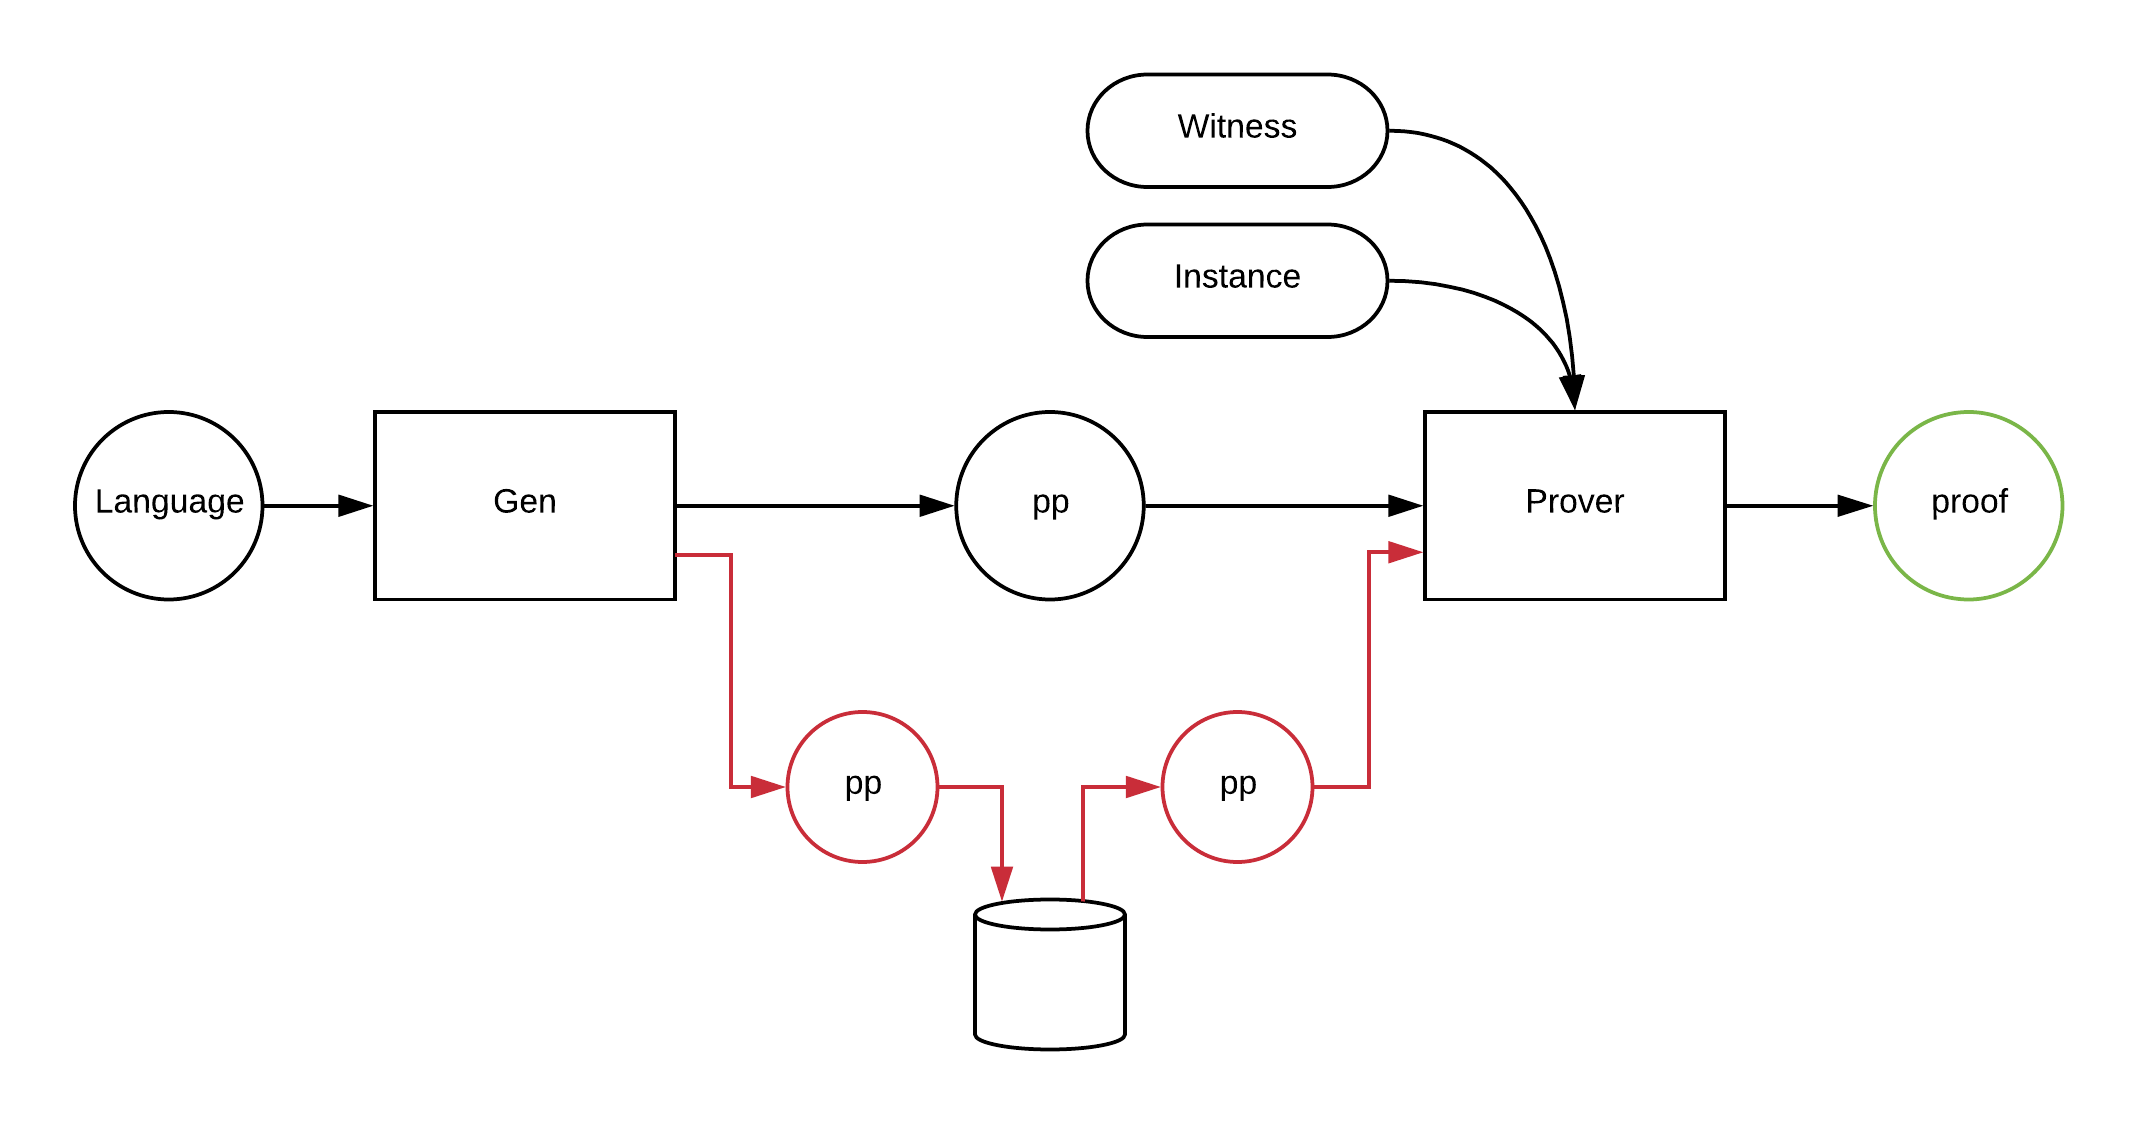
\includegraphics[width=\textwidth]{figs/implem--api-diagram.png}
\pdfcomment[author={Aur{\'e}lien Nicolas}]{the Verifier could appear here. \textCR\textCR PP, Instance, and Proof go into the Verifier box.}

{\centering \textbf{Figure \thefigure. }\tmpfigcap}
\end{center}
\end{figure}


We did not complete a generic API design for proving systems, but we did survey numerous tradeoffs and design approaches for such an API that may be of future value.

We separate the APIs and interfaces between the universal and non-universal NIZK setting. In the universal setting, the NIZK's CRS generation is independent of the relation (i.e., one CRS enables proving any NP statement). In the non-universal settings, the CRS generation depends on the relation (represented as a constraint system), and a given CRS enables proving the statements corresponding to any instance with respect to the specific relation.


\vspace{.5em}
\def\tmptabtitle{APIs and interfaces by types of universality and preprocessing}
{\mytabcap{\tmptabtitle}{\tmptabtitle}\label{tab:apps:APIS-and-interfaces-by-univ-and-preproc}}
\vspace{-1.5em}
\begin{longtable}{|>{\begmin{.30}}l<{\myendmini}|>{\begmin{.30}}l<{\myendmini}|>{\begmin{.30}}l|} %%%the last column ends with \rowend, which closes the minipage and adds \\
\hline 
	   & \textbf{Preprocessing} \\ (Generate has superpolylogarithmic runtime / output size as function of constraint system size)
		 & \textbf{Non-preprocessing} \\ (Generate runtime and output size is fast and CRS is at most polylogarithmic in constraint system size) \rowend
%%%%%%
\hline \textbf{Non-universal} \\ (Generate needs constraint system as input)
     & QAP-based \\ \cite{2013:SP:Pinocchio}, \cite{2013:Eurocrypt:quadratic-span-programs-and-succinct-NIZKs-without-PCPs}, \cite{2013:crypto:SNARKs-for-C}
		 & ? \rowend
%%%%%%
\hline {\textbf{Universal}} \\ (Generate needs just a size bound)
     & vnTinyRAM \\ vRAM \\ Bulletproofs (with explicit CRH)
		 & Bulletproofs (with PRG-based CRH generation) \rowend
%%%%%%
\hline \textbf{Universal and scalable}\\ (Generate needs nothing but security parameter)
		 & (impossible)
		 & ``Fully scalable'' SNARKs based on PCD (recursive composition) \rowend
\hline
\end{longtable}

In any case, we identified several capabilities that proving systems may need to express via a generic interface:

\begin{enumerate}
 \item The creation of CRS objects in the form of proving and verifying parameters, given the input language or size bound.
 \item The serialization of CRS objects into concrete encodings.
 \item Metadata about the proving system such as the size and characteristic of the field (for arithmetic constraints).
 \item Witness objects containing private inputs known only to the prover, and Instance objects containing public inputs known to the prover and verifier.
 \item The creation of Proof objects when supplied proving parameters, an Instance, and a Witness.
 \item The verification of Proof objects given verifying parameters and an Instance.
\end{enumerate}

\textbf{Future work:} 
We would like to see a concrete API design which leverages our tentative model, with additional work to encode concepts such as recursive composition and the batching of proving and verification operations.


%%%%%%%%%%%%%%%%%%%%%%%%%%%%%%
\subsection{R1CS File Format}

There are many frontends for constructing constraint systems, and many backends which consume constraint systems (and variable assignments) to create or verify proofs. We focused on creating a file format that frontends and backends can use to communicate constraint systems and variable assignments. Goals include simplicity, ease of implementation, compactness and avoiding hard-coded limits.

Our initial work focuses on R1CS due to its popularity and familiarity. 
Refer to the \hyperref[chap:track-security]{Security Track} document for more information about constraint systems. 
The design we arrived at is tentative and requires further iteration. 
Implementation and specification work will appear at \myurl{https://github.com/zkpstandard/file\_formats}.


\emph{R1CS (Rank 1 Constraint Systems)} is an NP-complete language for specifying relations as a system of bilinear constraints (i.e., a rank 1 quadratic constraint system), 
as defined in \cite[Appendix E in extended version]{2013:crypto:SNARKs-for-C}; %%%[BCGTV13, Appendix E in extended version]; 
this is a more intuitive reformulation of QAP \emph{QAP (Quadratic Arithmetic Program)}, 
defined in \cite{2013:SP:Pinocchio}. %%%[PHGR13]. 
R1CS is the native constraint system language of many ZK proof constructions (see the \hyperref[chap:track-security]{Security Track} document), including many ZK proof applications in operational deployment.

Our proposed format makes heavy use of variable-length integers which are prevalent in the (space-efficient) encoding of an R1CS. 
We refer to VarInt as a variable-length unsigned integer, and SignedVarInt as a variable-length signed integer. 
We typically use VarInt for lengths or version numbers, and SignedVarInt for field element constants. 
The actual description of a VarInt is not yet specified.

We’ll be working with primitive variable indices of the following form:

{\ttfamily
ConstantVar $\shortleftarrow$  SignedVarInt(0)\\
InstanceVar(i) $\shortleftarrow$  SignedVarInt(-(i + 1))\\
WitnessVar(i) $\shortleftarrow$  SignedVarInt(i + 1)\\
VariableIndex $\shortleftarrow$ ConstantVar / InstanceVar(i) / WitnessVar(i)
}

\emph{ConstantVar} represents an indexed constant in the field, usually assigned to one. 
\emph{InstanceVar} represents an indexed variable of the instance, or the public input, serialized with negative indices. 
\emph{WitnessVar} represents an indexed variable of the witness, or the private/auxiliary input, serialized with positive indices. 
\emph{VariableIndex} represents one of any of these possible variable indices.

We’ll also be working with primitive expressions of the following form:

{\ttfamily
Coefficient $\shortleftarrow$ SignedVarInt \\
Sequence(Entry) $\shortleftarrow$  | length: VarInt | length * Entry | \\
LinearCombination $\shortleftarrow$  Sequence(| VariableIndex | Coefficient |)
}
\begin{itemize}
    \item Coefficients must be non-zero.
    \item Entries should be sorted by type, then by index:
		\begin{itemize}
        \item | ConstantVar | sorted(InstanceVar) | sorted(WitnessVar) |
		\end{itemize}
\end{itemize}

{\ttfamily
Constraint $\shortleftarrow$  \\
| A: LinearCombination | B: LinearCombination | C: LinearCombination |
}

We represent a \emph{Coefficient} (a constant in a linear combination) with a \emph{SignedVarInt}. 
(TODO: there is no constraint on its canonical form.) These should never be zero. 
We express a \emph{LinearCombination} as sequences of \emph{VariableIndex} and \emph{Coefficient} pairs. 
Linear combinations should be sorted by type and then by index of the \emph{VariableIndex}; 
i.e., \emph{ConstantVar} should appear first, \emph{InstanceVar} should appear second (ascending) and \emph{WitnessVar} should appear last (ascending).

We express constraints as three \emph{LinearCombination} objects A, B, C, where the encoded constraint represents A * B = C.

The file format will contain a header with details about the constraint system that are important for the backend implementation or for parsing.

{\ttfamily
Header(version, vals) \shortleftarrow\\
| version: VarInt | vals: Sequence(SignedVarInt) |
}

The \emph{vals} component of the \emph{Header} will contain information such as:
\begin{itemize}
  \item  {\tt P} \shortleftarrow\ Field characteristic
  \item  {\tt D} \shortleftarrow\ Degree of extension
  \item  {\tt N\_X} \shortleftarrow\ Number of instance variables
  \item  {\tt N\_W} \shortleftarrow\ Number of witness variables
\end{itemize}

The representation of elements of extension fields is not currently specified, so {\tt D} should be 1.

The file format contains a magic byte sequence  “R1CSstmt”, a header, and a sequence of constraints, as follows:

{\ttfamily
R1CSFile \shortleftarrow\\
| "R1CSstmt" | Header(0, [ P, D, N\_X, N\_W, … ]) | Sequence(Constraint) |
}

Further values in the header are undefined in this specification for version 0, and should be ignored. The file extension “.r1cs” is used for R1CS circuits.

\textbf{Further work:} We wish to have a format for expressing the assignments for use by the backend in generating the proof. We reserve the magic “R1CSasig” and the file extention “.assignments” for this purpose. We also wish to have a format for expressing symbol tables for debugging. We reserve the magic “R1CSsymb” and the file extention “.r1cssym” for this purpose.

In the future we also wish to specify other kinds of constraint systems and languages that some proving systems can more naturally consume.



%%%%%%%%%%%%%%%%%%%%%%%%%%%%%%%%%%%%%%%%%%%%%%%%%%%%%%%%%%%%
%%%%%%%%%%%%%%%%%%%%%%%%%%%%%%%%%%%%%%%%%%%%%%%%%%%%%%%%%%%%
%%%\renewcommand{\thesection}{\hspace*{-1em}}

\section{Benchmarks}

As the variety of zero-knowledge proof systems and the complexity of applications has grown, it has become more and more difficult for users to understand which proof system is the best for their application. Part of the reason is that the tradeoff space is high-dimensional. Another reason is the lack of good, unified benchmarking guidelines. We aim to define benchmarking procedures that both allow fair and unbiased comparisons to prior work and also aim to give enough freedom such that scientists are incentivized to explore the whole tradeoff space and set nuanced benchmarks in new scenarios and thus enable more applications.\\
The benchmark standardisation is meant to document best practices, not hard requirements. They are especially recommended for new general-purpose proof systems as well as implementations of existing schemes. Additionally the long-term goal is to enable independent benchmarking on standardized hardware.


%%%%%%%%%%%%%%%%%%%%%%%%%%%%%%
\subsection{What metrics and components to measure}

We recommend that as the primary metrics the \textbf{running time (single-threaded)} and the \textbf{communication complexity} (proof size, in the case of non-interactive proof systems) of all components should be measured and reported for any benchmark. The measured components should at least include the \textbf{prover} and the \textbf{verifier}. If the setup is significant then this should also be measured, further system components like parameter loading and number of rounds (for interactive proof systems) are suggested.

The following metrics are additionally suggested:
\begin{itemize}[label={- }]
\item Parallelizability
\item Batching
\item Memory consumption (either as a precise measurement or as an upper bound)
\item Operation counts (e.g. number of field operations, multi-exponentiations, FFTs and their sizes)
\item Disk usage/Storage requirement
\item Crossover point: point where verifying is faster than running the computation
\item Largest instance that can be handled on a given system
\item Witness generation (this depends on the higher-level compiler and application)
\item Tradeoffs between any of the metrics.
\end{itemize}



%%%%%%%%%%%%%%%%%%%%%%%%%%%%%%
\subsection{How to run the benchmarks}
Benchmarks can be both of analytical and computational nature. Depending on the system either may be more appropriate or they can supplement each other. An analytical benchmark consists of asymptotic analysis as well as concrete formulas for certain metrics (e.g. the proof size). Ideally analytical benchmarks are parameterized by a security level or otherwise they should report the security level for which the benchmark is done, along with the assumptions that are being used.

Computational benchmarks should be run on a consistent and commercially available machine. The use of cloud providers is encouraged, as this allows for cheap reproducibility. The machine specification should be reported along with additional restrictions that are put on it (e.g. throttling, number of threads, memory supplied). Benchmarking machines should generally fall into one of the following categories and the machine description should indicate the category. If the software implementation makes certain architectural assumptions (such as use of special hardware instructions) then this should be clearly indicated.

\begin{itemize}[label={- }]
    \item Battery powered mobile devices
    \item Personal computers such as laptops
    \item Server style machines with many cores and large memories
    \item Server clusters using multiple machines 
    \item Custom hardware (should not be used to compare to software implementations)
\end{itemize}


We recommend that most runs are executed on a single-threaded machine, with parallelizability being an optional metric to measure. The benchmarks should be run at approximately \textbf{120}-bit security or larger. The conjectured security level, and whether it is in a post-quantum or classical setting, should be clearly stated.

In order to enable better comparisons we recommend that the metrics of other proof systems\slash implementations are also run on the same machine and reported. The onus is on the library developer to provide a simple way to run any instance on which a benchmark is reported.   This will additionally aid the reproducibility of results. Links to implementations will be gathered at zkp.science and library developers are encouraged to ensure that their library is properly referenced. Further we encourage scientific publishing venues to require the submission of source code if an implementation is reported. Ideally these venues even test the reproducibility and indicate whether results could be reproduced.


%%%%%%%%%%%%%%%%%%%%%%%%%%%%%%
\subsection{What benchmarks to run}
We propose a set of benchmarks that is informed by current applications of zero-knowledge proofs, as well as by differences in proving systems. This list in no way complete and should be amended and updated as new applications emerge and new systems with novel properties are developed. Zero-knowledge proof systems can be used in a black-box manner on an existing application, but often designing the application with a proof system in mind can yield large efficiency gains. To cover both scenarios we suggest a set of benchmarks that include commonly used primitives (e.g. SHA-256) and one where only the functionality is specified but not the primitives (e.g. a collision-resistant hash function at 120-bit classical security). 


\paragraph{Commonly used primitives.}

Here we list a set of primitives that both serve as microbenchmarks and are of separate interest. Library developers are free to choose how their library runs a given primitive, but we will aid the process by providing circuit descriptions in commonly used file formats (e.g. R1CS). 

Recommended
\begin{itemize}[label={- }]
    \item SHA-256
    \item AES
    \item A simple vector or matrix product at different sizes
\end{itemize}
Further suggestions
\begin{itemize}[label={- }]
    \item Zcash Sapling “spend” relation
    \item RC4 (for RAM memory access)
    \item Scrypt
    \item TinyRAM running for n steps with memory size s 
    \item Number theoretic transform (coefficients to points)
		\begin{itemize}[label={- }]
        \item Small fields 
        \item Big fields
        \item Pattern matching
		\end{itemize}
\end{itemize}


Repetition

The above relations, parallelized by putting $n$ copies in parallel.



\paragraph{Functionalities.}

The following are examples of cryptographic functionalities that are especially interesting to application developers. The realization of the primitive may be secondary, as long as it achieves the security properties. It is helpful to provide benchmarks for a constraint-system implementation of a realization of these primitives that is tailored for the NIZK backend.

In all of the following, the primitive should be given at a level of 120 bits or higher and match the security of the NIZK proof system.
\begin{itemize}
    \item Asymmetric cryptography
				\begin{itemize}[label={- }]
        \item Signature verification
        \item Public key encryption
        \item Diffie Hellman key exchange over any group with 128 bit security
				\end{itemize}
    \item Symmetric \& Hash
				\begin{itemize}[label={- }]
        \item Collision-resistant hash function on a 1024-byte message
        \item Set membership in a set of size $2^{20}$ (e.g., using Merkle authentication tree)
        \item MAC
        \item AEAD
				\end{itemize}
    \item The scheme’s own verification circuit, with matching parameters, for recursive composition (Proof-Carrying Data)
    \item Range proofs [Freely chosen commitment scheme]
				\begin{itemize}[label={- }]
        \item Proof that number is in $[0, 2^{64})$ 
        \item Proof that number is positive
				\end{itemize}
    \item Proof of permutation (proving that two committed lists contain the same elements)
\end{itemize}



%%%%%%%%%%%%%%%%%%%%%%%%%%%%%%
\subsection{Security}
When benchmarking it is important to compare the claimed and achieved security of different proof systems. To aid this benchmarks should make it clear which security level (Definition see theory track\luissug{Revise ``Security'' vs. ``Theory''?} document) is being used. 
In particular the benchmark should clearly state under which assumptions the claimed security is achieved. 
If the security is conjectured then benchmarks should display both the conjectured as well as the proven performance. 
Benchmarks should be run with at least 120-bit security. 
If the proof system claims to be quantum-resistant it should be clearly stated whether the benchmarks are in the classical or quantum setting. 
Further if the quantum setting is benchmarked, the benchmarked primitives should be adjusted as well.


%%%%%%%%%%%%%%%%%%%%%%%%%%%%%%%%%%%%%%%%%%%%%%%%%%%%%%%%%%%%
%%%%%%%%%%%%%%%%%%%%%%%%%%%%%%%%%%%%%%%%%%%%%%%%%%%%%%%%%%%%
\section{Correctness and Trust}

In this section we explore the requirements for making the implementation of the proof system trustworthy. Even if the mathematical scheme fulfills the claimed properties (e.g., it is proven secure in the requisite sense, its assumptions hold and security parameters are chosen judiciously), many things can go wrong in the subsequent implementation: code bugs, structured reference string subversion, compromise during deployment, side channels, tampering attacks, etc. This section aims to highlight such risks and offer considerations for practitioners.


%%%%%%%%%%%%%%%%%%%%%%%%%%%%%%
\subsection{Considerations}


\paragraph{Design of high-level protocol and statement.}

The specification of the high-level protocol that invokes the ZK proof system (and in particular, the NP statement to be proven in zero knowledge) may fail to achieve the intended domain-specific security properties.

Methodology for specifying and verifying these protocols is at its infancy, and in practice often relies on manual review and proof sketches. 
Possible methods for attaining assurance include reliance on peer-reviewed academic publications 
(e.g., Zerocash \cite{2014:SP:Zerocash} %[BCGGMT14] 
and Cinderella \cite{2016:SP:cinderella}) %[DFKP16]), 
reuse of high-level gadgets as discussed in the \hyperref[chap:track-apps]{Applications Track}, careful manual specification and proving of protocol properties by trained cryptographers, and emerging tools for formal verification.

Whenever nontrivial optimizations are applied to a statement, such as algebraic simplification, or replacement of an algorithm used in the original intended statement with a more efficient alternative, those optimizations should be supported by proofs at an appropriate level of formality.

See the \hyperref[chap:track-apps]{Applications Track} document for further discussion.


\paragraph{Choice of cryptographic primitives.}

Traditional cryptographic primitives (hash functions, PRFs, etc.) in common use are generally not designed for efficiency when implemented in circuits for ZK proof systems. Within the past few years, alternative "circuit-friendly" primitives have been proposed that may have efficiency advantages in this setting (e.g., LowMC and MiMC). We recommend a conservative approach to assessing the security of such primitives, and advise that the criteria for accepting them need to be as stringent as for the more traditional primitives.


\paragraph{Implementation of statement.}

The concrete implementation of the statement to be proven by the ZK proof system (e.g., as a Boolean circuit or an R1CS) may fail to capture the high-level specification. This risk increases if the statement is implemented in a low abstraction level, which is more prone to errors and harder to reason about.

The use of higher-level specifications and domain-specific languages (see the Front Ends section) can decrease the risk of this error, though errors may still occur in the higher-level specifications or in the compilation process.

Additionally, risk of errors often arises in the context of optimizations that aim to reduce the size of the statement (e.g., circuit size or number of R1CS constraints).

Note that correct statement semantics is crucial for security. Two implementations that use the same high-level protocol, same constraint system and compatible backends may still fail to correctly interoperate if their instance reductions (from high-level statement to the low-level input required by the backend) are incompatible -- both in completeness (proofs don’t verify) or soundness (causing false but convincing proofs, implying a security vulnerability).


\paragraph{Side channels.}
Developers should be aware of the different processes in which side channel attacks can be detrimental and take measure to minimize the side channels. These include:
\begin{itemize}[label={- }]
    \item SRS generation --- in some schemes, randomly sampled elements which are discarded can be used, if exposed, to subvert the soundness of the system.
    \item Assignment generation / proving --- the private auxiliary data can be exposed, which allows the attacker to understand the secret data used for the proof.
\end{itemize}


\paragraph{Auditing.}

First of all, circuit designers should provide a high-level description of their circuit and statement
alongside the low-level circuit, and explain the connections between them.             

The high-level description should facilitate auditing of the security properties of the protocol
being implemented, and whether these match the properties intended by the designers or that are likely to be expected by users.

If the low-level description is not expressed directly in code, then the correspondence between the code and the description should be clear enough to be checked in the auditing process, either manually or with tool support.

A major focus of auditing the correctness and security of a circuit implementation will be in verifying that the low-level description matches the high-level one. This has several aspects, corresponding to the security properties of a ZK proof system:
\begin{itemize}
    \item An instance for the low-level circuit must reveal no more information than an instance for the high-level statement. This is most easily achieved by ensuring that it is a canonical encoding of the high-level instance.
    \item It must not be possible to find an instance and witness for the low-level circuit that does not correspond to an instance and witness for the high-level statement.
\end{itemize}

At all levels of abstraction, it is beneficial to use types to clarify the domains and representations of the values being manipulated. Typically, a given proving system will not be able to *directly* represent all of the types of value needed for a given high-level statement; instead, the values will be encoded, for example as field elements in the case of R1CS-based proof systems. The available operations on these elements may differ from those on the values they are representing; for instance, field addition does not correspond to integer addition in the case of overflow.

An adversary who is attempting to prove an instance of the statement that was not intended to be provable, is not necessarily constrained to using instance and witness variables that correspond to these intended representations. Therefore, close attention is needed to ensuring that the constraint system explicitly excludes unintended representations.

There is a wide space of design tradeoffs in how the frontend to a proof system can help to address this issue. The frontend may provide a rich set of types suitable for directly expressing high-level statements; it may provide only field elements, leaving representation issues to the frontend user; it may provide abstraction mechanisms by which users can define new types; etc. Auditability of statements expressed using the frontend should be a major consideration in this design choice.

If the frontend takes a "gadget" approach to composition of statement elements, then it must be clear whether each gadget is responsible for constraining the input and/or output variables to their required types.


\paragraph{Testing.}
Methods to test constraint systems include:
\begin{itemize}[label={- }]
    \item Testing for failure - does the implementation accept an assignment that should not be accepted?
    \item Fuzzing the circuit inputs.
    \item Finding missing constraints - e.g., missing boolean constraints on variables that represent bits, or other missing type constraints.
    \item Finding dead constraints, and reporting them (instead of optimising out).
    \item Detection of unintended nondeterminism. For instance, given a partial fixed assignment, solve for the remainder and check that there is only one solution.
\end{itemize}

A proof system implementation can support testing by providing access, for test and debugging purposes, to the reason why a given assignment failed to satisfy the constraints. It should also support injection of values for instance and witness variables that would not occur in normal use (e.g. because they do not represent a value of the correct type). These features facilitate “white box testing”, i.e. testing that the circuit implementation rejects an instance and witness \emph{for the intended reason}, rather than incidentally. Without this support, it is difficult to write correct tests with adequate coverage of failure modes.


%%%%%%%%%%%%%%%%%%%%%%%%%%%%%%
\subsection{SRS Generation}

A prominent trust issue arises in proving systems which require a parameter setup process (structured reference string) that involves secret randomness. 
These may have to deal with scenarios where the process is vulnerable or expensive to perform security. 
We explore the real world social and technical problems that these setups must confront, such as air gaps, public verifiability, scalability, handing aborts, and the reputation of participants, and randomness beacons.

ZKP schemes require a URS (\emph{uniform} reference string) or SRS (\emph{structured} reference string) for their soundness and/or ZK properties. 
This necessitates suitable randomness sources and, in the case of a common reference string, a securely-executed setup algorithm. 
Moreover, some of the protocols create reference strings that can be reused across applications. 
We thus seek considerations for executing the setup phase of the leading ZKP scheme families, and for sharing of common resources.\\
This section summarizes an open discussion made by the participants of the Implementation Track, aiming to provide considerations for practitioners to securely generate a CRS.


\paragraph{SRS subversion and failure modes.}
Constructing the SRS in a single machine might fit some scenarios. 
For example, this includes a scenario where the verifier is a single entity --- the one who generates the SRS. 
In that scenario, an aspect that should be considered is subversion zero-knowledge --- a property of proving schemes allowing to maintain zero-knowledge, even if the SRS is chosen maliciously by the verifier.

Strategies for subversion zero knowledge include:
\begin{itemize}[label={- }]
    \item Using a multi-party computation to generate the SRS
    \item Adaptation of either \cite{2016:Eurocrypt:On-the-Size-of-Pairing-Based-Non-interactive-Arguments} %[Groth16] or 
		[PHGR13]
    \item Updatable SRS - the SRS is generated once in a secure manner, and can then be specialized to many different circuits, without the need to re-generate the SRS
\end{itemize}

There are other subversion considerations which are discussed in the ZKProof \hyperref[chap:track-security]{Security Track}.



\paragraph{SRS generation using MPC}

In order to reduce the need of trust in a single entity generating the SRS, it is possible to use a multi-party computation to generate the SRS. 
This method should ideally be secure as long as one participant is honest (per independent computation phase). 
Some considerations to strengthen the security of the MPC include:
\begin{itemize}[label={- }]
    \item Have as many participants as possible
				\begin{itemize}
        \item Diversity of participants; reduce the chance they will collude
        \item Diversity of implementations (curve, MPC code, compiler, operating system, language)
        \item Diversity of hardware (CPU architecture, peripherals, RAM)
						\begin{itemize}[label={- }]
            \item One-time-use computers
            \item GCP / EC2 (leveraging enterprise security)
						\end{itemize}
        \item If you are concerned about your hardware being compromised, then avoid side channels (power, audio/radio, surveillance)
            \begin{itemize}[label={- }]
						\item Hardware removal:
								\begin{itemize}[label={- }]
                \item Remove WiFi/Bluetooth chip
                \item Disconnect webcam / microphone / speakers
                \item Remove hard disks if not needed, or disable swap
								\end{itemize}
            \item Air gaps
						\end{itemize}[label={- }]
        \item Deterministic compilation
        \item Append-only logs
        \item Public verifiability of transcripts
        \item Scalability
        \item Handling aborts
        \item Reputation
			\end{itemize}
    \item Information extraction from the hardware is difficult
				\begin{itemize}[label={- }]
        \item Flash drives with hardware read-only toggle
				\end{itemize}
\end{itemize}

Some protocols (e.g., Powers of Tau) also require sampling unpredictable public randomness. Such randomness can be harnessed from proof of work blockchains or other sources of entropy such as stock markets. Verifiable Delay Functions can further reduce the ability to bias these sources [BBBF18]

\paragraph{SRS reusability}
For schemes that require an SRS, it may be possible to design an SRS generation process that allows the re-usability of a part of the SRS, thus reducing the attack surface. A good example of it is the \href{https://github.com/ebfull/powersoftau}{Powers of Tau} method for the \href{https://eprint.iacr.org/2016/260}{Groth16} construction, where most of the SRS can be reused before specializing to a specific constraint system.


\paragraph{Designated-verifier setting}
There are cases where the verifier is a known-in-advance single entity. There are schemes that excel in this setting. Moreover, schemes with public verifiability can be specialized to this setting as well.


%%%%%%%%%%%%%%%%%%%%%%%%%%%%%%
\subsection{Contingency plans}
We would like to explore in future workshops the notion of contingency plans. For example, how do we cope:
\begin{itemize}[label={- }]
    \item With our proof system being compromised? 
    \item With our specific circuit having a bug?  
    \item When our ZKP protocol has been breached  (identifying proofs with invalid witness, etc)
\end{itemize}
Some ideas that were discussed and can be expanded on are:
\begin{itemize}[label={- }]
    \item Scheme-agility and protocol-agility in protocols - when designing the system, allow flexibility for the primitives used
    \item Combiners (using multiple proof systems in parallel) - to reduce the reliance on a single proof system, use multiple
    \item Discuss ways to identify when ZKP protocol has been breached (identifying proofs with invalid witness, etc)
\end{itemize}


%%%%%%%%%%%%%%%%%%%%%%%%%%%%%%%%%%%%%%%%%%%%%%%%%%%%%%%%%%%%
%%%%%%%%%%%%%%%%%%%%%%%%%%%%%%%%%%%%%%%%%%%%%%%%%%%%%%%%%%%%
\section{Extended Constraint-System Interoperability}

The following are stronger forms of interoperability which have been identified as desirable by practitioners, and are to be addressed by the ongoing standardization effort.


%%%%%%%%%%%%%%%%%%%%%%%%%%%%%%
\subsection{Statement and witness formats}
In the R1CS File Format section and associated resources, we define a file format for R1CS constraint systems. There remains to finalize this specification, including instances and witnesses. This will enable users to have their choice of frameworks (frontends and backends) and streaming for storage and communication, and facilitate creation of benchmark test cases that could be executed by any backend accepting these formats.
 
Crucially, analogous formats are desired for constraint system languages other than R1CS.


%%%%%%%%%%%%%%%%%%%%%%%%%%%%%%
\subsection{Statement semantics, variable representation \& mapping}

Beyond the above, there’s a need for different implementations to coordinate the semantics of the statement (instance) representation of constraint systems. For example, a high-level protocol may have an RSA signature as part of the statement, leaving ambiguity on how big integers modulo a constant are represented as a sequence of variables over a smaller field, and at what indices these variables are placed in the actual R1CS instance.

Precise specification of statement semantics, in terms of higher-level abstraction, is needed for interoperability of constraint systems that are invoked by several different implementations of the instance reduction (from high-level statement to the actual input required by the ZKP prover and verifier). One may go further and try to reuse the actual implementation of the instance reduction, taking a high-level and possibly domain-specific representation of values (e.g., big  integers) and converting it into low-level variables. This raises questions of language and platform incompatibility, as well as proper modularization and packaging.

Note that correct statement semantics is crucial for security. Two implementations that use the same high-level protocol, same constraint system and compatible backends may still fail to correctly interoperate if their instance reductions are incompatible -- both in completeness (proofs don’t verify) or soundness (causing false but convincing proofs, implying a security vulnerability). Moreover, semantics are a requisite for verification and helpful for debugging.

Some backends can exploit uniformity or regularity in the constraint system (e.g., repeating patterns or algebraic structure), and could thus take advantage of formats and semantics that convey the requisite information.

At the typical complexity level of today’s constraint systems, it is often acceptable to handle all of the above manually, by fresh re-implementation based on informal specifications and inspection of prior implementation. We expect this to become less tenable and more error prone as application complexity grows.

%%%%%%%%%%%%%%%%%%%%%%%%%%%%%%
\subsection{Witness reduction}

Similar considerations arise for the witness reduction, converting a high-level witness representation (for a given statement) into the assignment to witness variables. For example, a high-level protocol may use Merkle trees of particular depth with a particular hash function, and a high-level instance may include a Merkle authentication path. The witness reduction would need to convert these into witness variables, that contain all of the Merkle authentication path data (encoded by some particular convention into field elements and assigned in some particular order) and moreover the numerous additional witness variables that occur in the constraints that evaluate the hash function, ensure consistency and Booleanity, etc.

The witness reduction is highly dependent on the particular implementation of the constraint system. Possible approaches to interoperability are, as above: formal specifications, code reuse and manual ad hoc compatibility.

%%%%%%%%%%%%%%%%%%%%%%%%%%%%%%
\subsection{Gadgets interoperability}
At a finer grain than monolithic constraint systems and their assignments, there is need for sharing subcircuits and gadgets. For example, libsnark offers a rich library of highly optimized R1CS gadgets, which developers of several front-end compilers would like to reuse in the context of their own constraint-system construction framework.

While porting chunks of constraints across frameworks is relatively straightforward, there are challenges in coordinating the semantics of the externally-visible variables of the gadget, analogous to but more difficult than those mentioned above for full constraint systems: there is a need to coordinate or reuse the semantics of a gadget’s externally-visible variables, as well as to coordinate or reuse the witness reduction function of imported gadgets in order to converts a witness into an assignment to the internal variables.

As for instance semantics, well-defined gadget semantics is crucial for soundness, completeness and verification, and is helpful for debugging.

%%%%%%%%%%%%%%%%%%%%%%%%%%%%%%
\subsection{Procedural interoperability}
An attractive approach to the aforementioned needs for instance and witness reductions (both at the level of whole constraint systems and at the gadget level) is to enable one implementation to invoke the instance/witness reductions of another, even across frameworks and programming languages.

This requires communication not of mere data, but invocation of procedural code. Suggested approaches to this include linking against executable code (e.g., .so files or .dll), using some elegant and portable high-level language with its associated portable, or using a low-level portable executable format such as WebAssembly. All of these require suitable calling conventions (e.g., how are field elements represented?), usage guidelines and examples.

Beyond interoperability, some low-level building blocks (e.g., finite field and elliptic curve arithmetic) are needed by many or all implementations, and suitable libraries can be reused. To a large extent this is already happening, using the standard practices for code reuse using native libraries. Such reused libraries may offer a convenient common ground for consistent calling conventions as well.

%%%%%%%%%%%%%%%%%%%%%%%%%%%%%%
\subsection{Proof interoperability}
Another desired goal is interoperability between provers and verifiers that come from different implementations, i.e., being able to independently write verifiers that make consistent decisions and being able to re-implement provers while still producing proofs that convince the old verifier.

This is especially pertinent in applications where proofs are posted publicly, such as in the context of blockchains (see the Applications Track document), and multiple independent implementations are desired for both provers and verifiers.

To achieve such interoperability between provers and verifiers, they must agree on all of the following:
\begin{itemize}
    \item ZK proof system (including fixing all degrees of freedom, such as choice of finite fields and elliptic curves)
    \item Instance and witness formats (see above subsection)
    \item Prover parameters formats
    \item Verifier parameters formats
    \item Proof formats
    \item A precise specification of the constraint system (e.g., R1CS) and corresponding instance and witness reductions (see above subsection).
\end{itemize}

Alternatively: a precise high-level specification along with a precisely-specified, deterministic frontend compilation.


%%%%%%%%%%%%%%%%%%%%%%%%%%%%%%
\subsection{Common reference strings}
There is also a need for standardization regarding Common Reference String (CRS), i.e., prover parameters and verifier parameters. First, interoperability is needed for streaming formats (communication and storage), and would allow application developers to easily switch between different implementations, with different security and performance properties, to suit their need. Moreover, for Structured Reference Strings (SRS), there are nontrivial semantics that depend on the ZK proof system and its concrete realization by backends, as well as potential for partial reuse of SRS across different circuits in some schemes (e.g., the Powers of Tau protocol). 


%%%%%%%%%%%%%%%%%%%%%%%%%%%%%%%%%%%%%%%%%%%%%%%%%%%%%%%%%%%%
%%%%%%%%%%%%%%%%%%%%%%%%%%%%%%%%%%%%%%%%%%%%%%%%%%%%%%%%%%%%
\section{Future goals}


%%%%%%%%%%%%%%%%%%%%%%%%%%%%%%
\subsection{Interoperability}

Many additional aspects of interoperability remain to be analyzed and supported by standards, to support additional ZK proof system backends as well as additional communication and reuse scenarios. Work has begun on multiple fronts both, and a dedicated public \href{https://groups.google.com/a/zkproof.org/forum/\#!forum/interoperability}{mailing list} is established.

\paragraph{Additional forms of interoperability.}
As discussed in the Extended Constraint-System Interoperability section above, even within the R1CS realm, there are numerous additional needs beyond plain constraint systems and assignment representations. These affect security, functionality and ease of development and reuse.


\paragraph{Additional relation styles.}
The R1CS-style constraint system has been given the most focus in the Implementation Track discussions in the first workshop, leading to a file format and an API specification suitable for it. It is an important goal to discuss other styles of constraint systems, which are used by other ZK proof systems and their corresponding backends. This includes arithmetic and Boolean circuits, variants thereof which can exploit regular/repeating elements, as well as arithmetic constraint satisfaction problems.


\paragraph{Recursive composition.}
The technique of recursive composition of proofs, and its abstraction as Proof-Carrying Data (PCD) [CT10][BCTV14], can improve the performance and functionality of ZK proof systems in applications that deal with multi-stage computation or large amounts of data. This introduces additional objects and corresponding interoperability considerations. For example, PCD compliance predicates are constraint systems with additional conventions that determine their semantics, and for interoperability these conventions require precise specification.


\paragraph{Benchmarks.}
We strive to create concrete reference benchmarks and reference platforms, to enable cross-paper milliseconds comparisons and competitions.

We seek to create an open competition with well-specified evaluation criteria, to evaluate different proof schemes in various well-defined scenarios.



%%%%%%%%%%%%%%%%%%%%%%%%%%%%%%
\subsection{Frontends and DSLs}
We would like to expand the discussion on the areas of domain-specific languages, specifically in aspects of interoperability, correctness and efficiency (even enabling source-to-source optimisation).

The goal of Gadget Interoperability, in the Extended Constraint-System Interoperability section, is also pertinent to frontends.



%%%%%%%%%%%%%%%%%%%%%%%%%%%%%%
\subsection{Verification of implementations}
We would to discuss the following subjects in future workshops, to assist in guiding towards best practices: formal verification, auditing, consistency tests, etc.



%%%%%%%%%%%%%%%%%%%%%%%%%%%%%%%%%%%%%%%%%%%%%%%%%%%%%%%%%%%%
%%%%%%%%%%%%%%%%%%%%%%%%%%%%%%%%%%%%%%%%%%%%%%%%%%%%%%%%%%%%
\paragraph{List of references:}
\pdfbookmark[1]{List of references}{pdfbkm:implem:list-refs}
\cite{2018:crypto:VDFs},
\cite{2014:SP:Zerocash},
\cite{2013:crypto:SNARKs-for-C},
\cite{2014:crypto:Scalable-Zero-Knowledge-via-Cycles-of-Elliptic-Curves},
\cite{2010:ICS:proof-carrying-data},
\cite{2016:SP:cinderella},
\cite{2016:Eurocrypt:On-the-Size-of-Pairing-Based-Non-interactive-Arguments},
\cite{2013:Eurocrypt:quadratic-span-programs-and-succinct-NIZKs-without-PCPs},
\cite{2013:SP:Pinocchio}.

